\begin{frame}
  \frametitle{Organización física de un \textbf{HDD}}
  \begin{figure}
    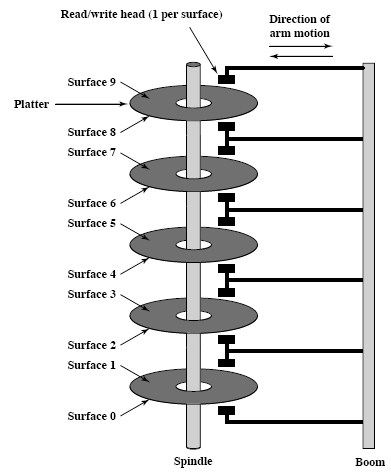
\includegraphics[scale=0.4]{images/disk1.png}
  \end{figure}
\end{frame}

\begin{frame}
  \frametitle{Organización física de un \textbf{HDD} (cont.)}
  \begin{figure}
    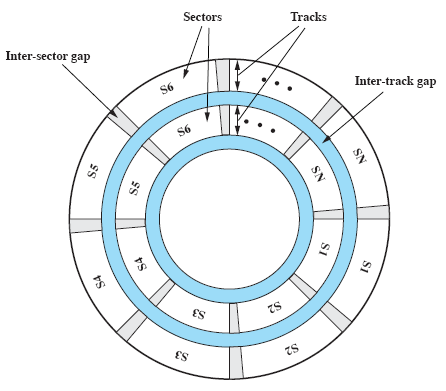
\includegraphics[scale=0.4]{images/disk2.png}
  \end{figure}
\end{frame}

\begin{frame}
  \frametitle{Organización física de un \textbf{HDD} (cont.)}
  \begin{itemize}
  	\item Cilindro N: todas las n-esimas pistas de todas las caras
  \end{itemize}
  \begin{figure}
    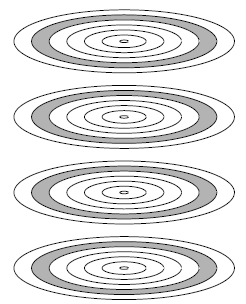
\includegraphics[scale=0.4]{images/cylinders.png}
  \end{figure}
\end{frame}

\begin{frame}
  \frametitle{Capacidad de un disco}
  \begin{itemize}
  	\item La capacidad de un disco esta dada por el producto de:
  	\begin{itemize}
  		\item Cantidad de caras: \emph{W}
  		\item Cantidad de pistas: \emph{X}
  		\item Cantidad de sectores por pista: \emph{Y}
  		\item Tamaño de sector: \emph{Z}
  	\end{itemize}

  	\emph{capadidad = W * X * Y * Z}
  \end{itemize}
\end{frame}

\begin{frame}
  \frametitle{Acceso a un disco}
  \begin{itemize}
  	\item Para realizar una \emph{E/S}, por ejemplo un acceso a disco, se requiere de una llamada al sistema (\textit{System Call}). En la misma se especifica:
  	\begin{itemize}
  		\item Tipo de operación (\emph{E} o \emph{S})
  		\item Dirección en disco para la transferencia (file descriptor que se obtuvo al abrir un archivo)
  		\item Dirección en memoria para la transferencia (de donde se lee o escribe)
  		\item Número de \bytes a transferir
  	\end{itemize}
  	\item Este requerimiento es pasado, por el \textit{kernel}, al subsistema de \emph{E/S} quien lo traduce en: \textbf{(\#Cara, \#Cilindro, \#Sector)}
  \end{itemize}
\end{frame}

\begin{frame}
  \frametitle{Tiempo de acceso a un disco}
  \begin{itemize}
    \item El tiempo de acceso esta dado por:
    \begin{itemize}
      \item \textbf{Seek time} (posicionamiento): tiempo que tarda en posicionarse la cabeza en el cilindro 
      \item \textbf{Latency time} (latencia): tiempo que sucede desde que la cabeza se posiciona en el cilindro hasta que el sector en cuestión pasa por debajo de la misma
      \item \textbf{Transfer time} (transferencia): tiempo de transferencia del sector (bloque) del disco a la memoria
    \end{itemize}    
  \end{itemize}
  \begin{figure}
      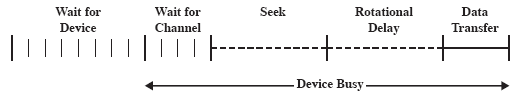
\includegraphics[scale=0.4]{images/dat.png}
  \end{figure}
\end{frame}

\begin{frame}
  \frametitle{Tiempo de acceso a un disco (cont.)}
  \begin{figure}
      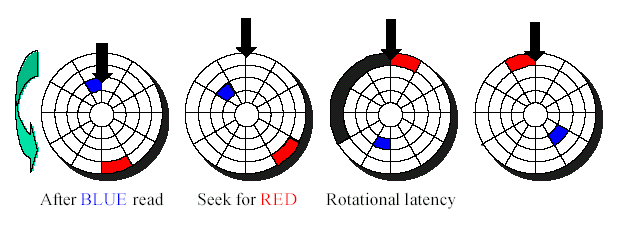
\includegraphics[scale=0.5]{images/dat2.png}
  \end{figure}
\end{frame}

\begin{frame}
  \frametitle{Tiempo de acceso a un disco (cont.)}
  \begin{itemize}
    \item \emph{Latency time} $\rightarrow$ si este tiempo no se conoce, se considera que es igual a lo que tarda el disco en dar media vuelta
    \item Ejemplo. Disco de 5400 \rpm $\rightarrow$
      \linebreak
      \linebreak
      \hspace{35pt} 5400 \_\_\_\_\_\_\_\_\_\_ 1' = 60'' = 60000 \ms 
      \linebreak  
      \hspace{35pt} 1/2  \_\_\_\_\_\_\_\_\_\_\_ x = 5,5 \ms    
  \end{itemize}
\end{frame}

%%%%%%%%%%%%%%%%%%%%%%%%%%%%%%%%%%%%%%%%%%%%%%%%%%%%%%%%%%%%%%%%%%

\begin{comment}

\begin{frame}[fragile]
  \frametitle{Características - Configuración de discos (cont.)}
  \begin{itemize}
	  \item A futuro, todos los dispositivos llamados hdX serán denominados sdX $\leftarrow$ Introducido en Debian/Squeeze
	  \item Por estas y otras razones se adoptan 4 mecanismos nuevos para nomenclar\footnote{\url{http://wiki.debian.org/Part-UUID}}:
	  \begin{itemize}
	  	\item Nombres persistentes por \textbf{UUID} (\small{Universal Unique Identifier}):
	  	\begin{lstlisting}
$ ls –l /dev/disk/by-uuid/
2d781b26-0285-421a-b9d0-d4a0d3b55680 -> ../../sda1
31f8eb0d-612b-4805-835e-0e6d8b8c5591 -> ../../sda7
		\end{lstlisting}
		\item Utilizando \textbf{labels}
		\begin{lstlisting}
$ ls -l /dev/disk/by-label
data -> ../../sdb2
data2 -> ../../sda2
		\end{lstlisting}
	  \end{itemize}
  \end{itemize}
\end{frame}

\begin{frame}
  \frametitle{Herramientas para particionar}
  \begin{itemize}
	  \item El particionado de un disco se lo puede realizar mediante:
	  \begin{itemize}
	  	\item Software destructivo: \textit{fdisk}
	  	\item Software no destructivo: \textit{fips}, \textit{gparted}
		\begin{figure}
		    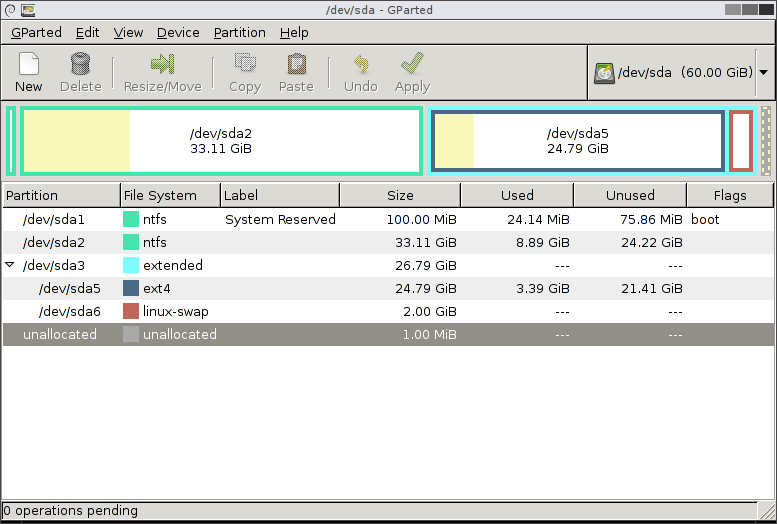
\includegraphics[scale=0.3]{images/gparted.png}
		\end{figure}
	  \end{itemize}
  \end{itemize}
\end{frame}

\begin{frame}[fragile]
  \frametitle{Permisos}
  \begin{itemize}
	  	\item Se aplican a directorios y archivos
	  	\item Existen 3 tipos de permisos y se basan en una notación octal:
	  	\begin{table}
		      \centering
		      \resizebox{10pc}{!}{
			  \begin{tabular}{| c | c | c |}
			      \hline
			      \bf Permiso & \bf Valor & \bf Octal \\
			      \hline
			      Lectura & R & 4 \\
			      \hline
			      Escritura & W & 2 \\
			      \hline
			      Ejecución & X & 1 \\
			      \hline
			  \end{tabular}
		      }
		\end{table}
		\item Se aplican sobre los usuarios:
		\begin{itemize}
			\item Usuario: permisos del dueño $\rightarrow$ \textbf{U}
			\item Usuario: permisos del grupo $\rightarrow$ \textbf{G}
			\item Usuario: permisos de otros usuario $\rightarrow$ \textbf{O}
		\end{itemize}
		\item Se utiliza el comando \textbf{chmod}:
		\begin{lstlisting}
$ chmod 755 /tmp/script
		\end{lstlisting}
  \end{itemize}
\end{frame}
\end{comment}